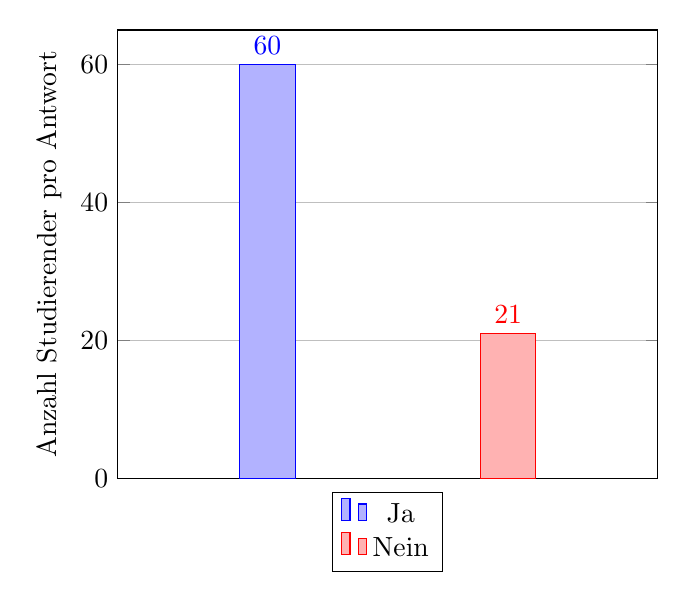
\begin{tikzpicture}
    \begin{axis}[
        x tick label style={
            /pgf/number format/1000 sep=},
        ylabel=Anzahl Studierender pro Antwort,
        enlarge x limits=1,
        ymax=65,
        ymin=0,
        legend style={at={(0.5,-0.03)},
        anchor=north,legend columns=1},
        ybar,
        bar width=20pt,
        xtick=\empty,
        xticklabels={},
        nodes near coords,
        grid=major,
    ]
    
    \addplot coordinates {(1,60)}; % Ja
    \addplot coordinates {(2,21)}; % Nein
    
    \legend{Ja, Nein}
    \end{axis}
\end{tikzpicture}